\section{MIMO in Handsets}
\label{sec:mimo_in_handsets}
Multiple antennas in both transmitter and receiver in wireless systems, which is better known as MIMO, has become a widespread technology and used in many applications today, due to its ability to increase performance. Most wireless systems are limited by the channel in which they propagate, due to phenomenons such as multi-path fading. Multi-path happens when the transmitted signal travels through multiple different paths, which influences the time it takes for the signal to reach the receiver, the angle of arrival, and even frequency shifts due to Doppler. This creates random fluctuation in the received signal level, affecting the performance of the wireless communication. MIMO is an effective way of dealing with the challenges in delivering more throughput and coupe with the multipath effects from buildings. MIMO exploits the multi-path phenomenon to transmit several different data streams simultaneously, also referred to as spatial multiplexing. This can help in both single user or in multi-user scenarios. For the single user, it allows for faster data rates without increasing the transmit power or allocating more frequency resources. In the multi-user scenario, the base station can effectively create beams to individual users while using the same shared frequency. This is also known as Space Division Multiple Access (SDMA). The purpose of this section is to explain what is understood by such a system, how it relates to the antenna design, and how it makes a difference. The principal mechanisms and performance metrics are explained. This section will not describe the statistical channel models but rather focus on the antenna related perspectives. 

\begin{figure}[htbp]
  \centering
  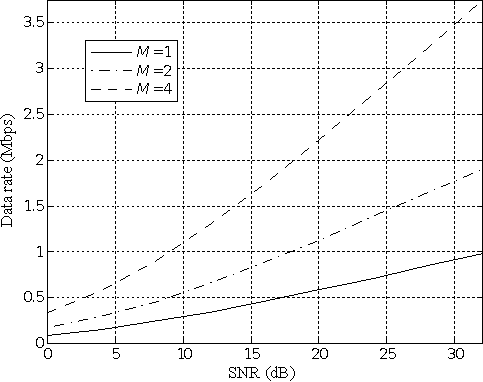
\includegraphics[scale=1.2]{img/analysis/datarateMimo}
  \caption{Throughput versus SNR given a specific M-ary MIMO-setup \cite{Ezio2007MIMO}.}
  \label{fig:mimo-throughput}
\end{figure}

\subsection{Perks of MIMO} 
As shown in the introduction to this section, the use of MIMO results in enhanced performance. Figure~\ref{fig:mimo-throughput} shows the general performance increase, however this is gained by the addition of multiple different performance gains. The performance gains are spatial diversity gain, multiplexing gain, array gain, and interference reduction \cite{Ezio2007MIMO}, which will be described briefly in the following.

\subsubsection{Spatial Diversity Gain}
The spatial diversity gain improves the resistance to fading in the receiver. This is done by providing the receiver with multiple different copies of the same transmitted signal. Ideally, the copies are independent from another. A diversity technique is required to combine the signals at the receiver \cite{Ezio2007MIMO}. Some examples could be equal gain combining, maximal-ratio combining, or selection combining. The spatial diversity is also quite intuitive since the probability that one of the signals are not in a fade increases per added element, given that they are somewhat independent. 
 
\subsubsection{Spatial Multiplexing Gain}
Spatial multiplexing can be used in scatter rich channels where the received signals are independent. Instead of transmitting the same signal, as done in diversity gain, the spatial multiplexing transmits multiple independent data streams. This allows for a linear increase in the data rate, thus the capacity of the wireless network is increased. Generally, the number of independent streams that can be supported is limited by the number of receive antennas \cite{Tim2012Practical}.

\subsubsection{Array Gain}
The array gain is the result of coherent combining of the wireless signals at the receiver, which results in an increase in the receive SNR. The array gain is improved linearly as the number of receive antennas increases \cite{tse2005fundamentals}. This gain improves the resistance to noise and thus also the coverage \cite{Tim2012Practical}.
  
\subsubsection{Interference Gain}
By using MIMO, the interference from different users and base stations can be avoided by exploiting extra spatial degrees of freedom, such as array gain. Furthermore, beam-steering could be implemented such that the signal could be directed towards the designated receiver. Obviously, all of the above can not be used at the same time. However, using a combination allows for improved coverage, capacity, and reliability \cite{Tim2012Practical}.

\subsection{Channel Capacity}
\def\snr{\text{SNR}_{\text{AWGN}}}
\def\PP{\overline{P}}
\def\CC{C_{\text{AWGN}}}

The capacity of a channel is the maximal transmission rate for which a reliable communication can be achieved, and if the transmission rate exceeds this, the system breaks down \cite{Tim2012Practical}. The channel capacity is one of the primary performance measures to characterize the performance of MIMO systems \cite{Tim2012Practical}. This section will focus on the capacity for time-invariant SISO, SIMO, MISO, and MIMO channels. The main assumptions for the time-invariant channel is the following \cite{Tim2012Practical}: 
\begin{itemize}
\item The channel is time-invariant.
\item A codeword spans over an asymptotic long data block, which averages out the noise.
\item Channel state information is available at both the transmitter and receiver. 
\end{itemize}

\subsubsection{Time-Invariant SISO Channel}
A simple SISO channel, as illustrated in Figure~\ref{fig:sisoModel}, is given by the input-output relation:
\begin{align*} %%
  y(k) = h x(k) + n(k)
\end{align*}

Here $h$ describes the channel, which is time \emph{independent}. The signal power is $\PP |h|^2$, which is the power in $h x(k)$ and the noise power of $n(k)$ is $\sigma_n^2$. Thus, the SNR is given by the ratio \cite{Tim2012Practical}
\begin{align} %%
  \snr = \frac{\PP |h|^2}{\sigma_n^2}
\end{align}
This yields a channel capacity of \cite{Tim2012Practical} 
\begin{align} %%
      \CC &= \log_2 \left( 1 + \snr \right)
\end{align}
It is seen that the SNR is an important factor for the AWGN channel capacity.
\begin{figure}[hbp]
  \centering
  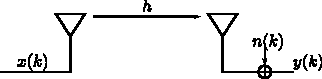
\includegraphics[scale=1.2]{img/analysis/sisoModel}
  \caption{The time-invariant SISO channel}
  \label{fig:sisoModel}
\end{figure}

\subsubsection{Time-Invariant SIMO Channel}
The channel capacity for a SIMO system, where a symbol $x(k)$ is sent from a single antenna and received at $M_R$ antennas, is illustrated in Figure~\ref{fig:simoModel}. In a SIMO system, the signal is coherently combined at the receiver. When including this post-processing, the system transforms into an equivalent SISO channel \cite{Tim2012Practical}.

\begin{figure}[htbp]
  \centering
  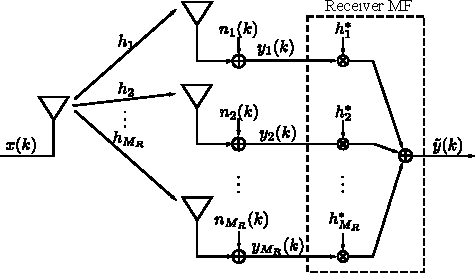
\includegraphics[scale=1.2]{img/analysis/simoModel}
  \caption{The time-invariant SIMO channel.}
  \label{fig:simoModel}
\end{figure}

The system model changes from a scalar equation to a vector notation due to the multiple antennas. The channel coefficients are denoted as $h_j$, $j,\ldots,M_R$ and are known at the transmitter. At a given antenna, $j$, the received signal $y_j(k)$ is given by \cite{Tim2012Practical}: 
\begin{align} %%
  y_j(k) = h_j x(k) + n_j(k)
\end{align}

The multiple antennas receive multiple distorted copies of the transmitted symbol. Each received signal, has different parts of the signal depending on the channel. To recover most of the original message, the different symbols are combined. This combination can be done in multiple ways: Matched filtering, maximum ratio combining, or equal-gain combining. Matched filtering requires the most amount of post-processing since it requires the signals to be aligned in phase, so they can be added constructively and scaled. This maximizes the post-processing SNR of the SIMO system. Mathematically the received signal at antenna $j$ is first multiplied with a scalar coefficient $h_j^*$ matched to the channel. This yields $|h_j|^2 x(k) + h_j^* n_j(k)$. The processed signals are then added up, resulting in a processed signal \cite{Tim2012Practical} 
\begin{align}%%
  \tilde{y}(k) = \norm{\mathbf{h}}^2 x(k) + \tilde{n}(k)
\end{align}

The SIMO system becomes equivalent to a scalar AWGN channel, with a potentially larger SNR due to the post-processing \cite{Tim2012Practical}. This leads us to an SNR and a channel capacity given by \cite{Tim2012Practical}
\begin{align} %%
\text{SNR}^{\text{TI}}_{\text{SIMO}} &= \frac{\PP \norm{\mathbf{h}}^2}{\sigma^2_n} \\
C^{\text{TI}}_{\text{SIMO}} &= \log_2 \left( 1+\frac{\PP \norm{\mathbf{h}}^2}{\sigma^2_n} \right)  
\end{align}

\subsubsection{Time-Invariant MISO Channel}
In the MISO case, the system consists of multiple antennas at the transmitter and a single antenna at the receiver. This is illustrated in Figure~\ref{fig:misoModel}.
\begin{figure}[htbp]
  \centering
  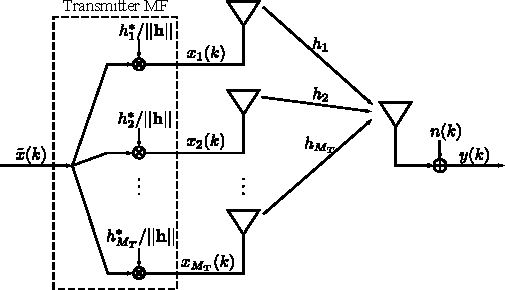
\includegraphics[scale=1.2]{img/analysis/misoModel}
  \caption{The time-invariant MISO channel.}
  \label{fig:misoModel}
\end{figure}
Given that the channel is known at the transmitter, it is possible to perform pre-processing on the transmitted signals. This transforms the MISO case in to an equivalent SISO channel. The pre-processing consists of scaling each version of the transmitted symbol to insure that the signals are added up constructively at the receiver. The pre-processing must take the channel for each antenna into account when doing this scaling. 

A signal $x_i(k)$ is sent from the $i$th antenna in the array. This signal travels through the channel $h_i$ and this channel is known at the transmitter. The received signal is then given as \cite{Tim2012Practical}: 
\begin{align}%%
  y(k) = \sum_{i=1}^{M_T} h_ix_i(k) + n(k) = \mathbf{h}^\intercal \mathbf{x}(k) + n(k)
\end{align}
where
\begin{where}
  \item[$M_T$] The number of transmitter antennas.
  \item[$\mathbf{h}$] $[h_1 \cdots h_{M_T}]^T$.
  \item[$\mathbf{x}$] $[x_1(k) \cdots x_{M_T}(k)]^T$.
\end{where}

The MISO becomes an equivalent SISO channel. The pre-processing that is often used is transmit spatial matched filtering or transmit MRC, where the transmitted signal is matched to the channel $h_i$ before being sent from antenna $i$. The weights applied in the transmit MF are the exact same as the receiver MF due to perfect knowledge of the channel \cite{Tim2012Practical}. The output of the pre-processing is under the power constraint $\sum_{i=1}^{M_T} E|x_i(k)|^2 \leq \PP$. The signal $x_i$ sent from the antenna is then \cite{Tim2012Practical}
\begin{align}%%
  x_i(k) = \frac{h_i^*}{\norm{\mathbf{h}} \tilde{x}(k)}
\end{align}

On the receiving side, the signals are phase-aligned and added constructively. It is obvious that more power is allocated to the stronger channels, thus maximizing the SNR. The SNR and channel capacity then becomes \cite{Tim2012Practical}:
\begin{align} %%
\text{SNR}^{\text{TI}}_{\text{MISO}} &= \frac{\PP \norm{\mathbf{h}}^2}{\sigma^2_n} \\
C^{\text{TI}}_{\text{MISO}} &= \log_2 \left( 1+\frac{\PP \norm{\mathbf{h}}^2}{\sigma^2_n} \right)  
\end{align}
Thus, it is seen that for time-invariant channels with perfect channel knowledge for both transmitter and receiver, the capacity for SIMO and MISO systems are the same. This is, however, not the case for fading channels when the channel state is unknown for the transmitter. This leads to performance degradation in the MISO case \cite{Tim2012Practical}. 

\subsubsection{Time-Invariant MIMO Channel}
When multiple antennas are available at both transmitter and receiver, the capacity can be increased by sending multiple symbols per transmission period. This relies on pre- and post-processing which is matched to singular value decomposition of the channel \cite{Tim2012Practical}, illustrated in Figure~\ref{fig:mimoModel}. This processing extracts independent spatial routes for the communication. MIMO can be interpreted as multiple pairs of independent SISO channels where the capacity simply becomes the sum of these independent SISO channels \cite{Tim2012Practical}.

\begin{figure}[htbp]
  \centering
  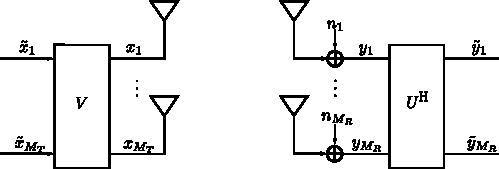
\includegraphics[scale=1.2]{img/analysis/mimoModel}
  \caption{The time-invariant MIMO channel.}
  \label{fig:mimoModel}
\end{figure}

The singular value decomposition of the channel matrix is fundamental in understanding the underlying concepts of MIMO systems. The SVD extracts the equivalent independent AWGN channels, gives the maximum number of streams that can be multiplexed, and it provides a simple way to compute the capacity. The SVD of the channel matrix $\mathbf{H}$ is \cite{Tim2012Practical}
\begin{align}%%
  \mathbf{H} = \mathbf{U} \Lambda \mathbf{V}^{\mathsf{H}} 
\end{align}
 
Both $\mathbf{U}$ ($M_R \times \ M_R$) and $\mathbf{V}$ ($M_T \times \ M_T$) are unitary matrices, and $\Lambda$ is a  $M_R \times \ M_T$ diagonal matrix with non-negative singular values $\lambda_k$ with $k=1, \cdots, M_{\text{min}}$ where $M_{\text{min}} = \min(M_T,M_R)$. The $\lambda_k$'s are called the eigenmodes of the channel and are often ordered decreasingly for convenience.

Another important quantity is the channel matrix rank $\mathbf{H}$, which is denoted $r_H$. This is defined as the number of nonzero singular values of $\mathbf{H}$, which determines the maximum number of independent streams that can be multiplexed at the same time \cite{Tim2012Practical}. The singular value and channel energy relationship is also useful. This is given as 
\begin{align} %%
  \text{tr}(\mathbf{H} \mathbf{H}^{\mathsf{H}}) = \sum_{i=1}^{M_T} \sum_{j=1}^{M_R} |h_{ji}|^2 = \sum_{k=1}^{r_H} \lambda_i^2
\end{align}
Each channel is called an eigenchannel. The entire MIMO channel is equivalent to the set of eigenchannels, each with a different SNR. Looking at the input-output relation \cite{Tim2012Practical}
\begin{align}%%
  \tilde{y} = \Lambda\mathbf{ \tilde{x}} + \mathbf{\tilde{n}}
\end{align}
From each input-output relation $\tilde{y}_k = \lambda_k \tilde{x}_k + \tilde{n}_k$ it is obvious that this describes an AWGN channel as seen previously in the SISO case. Since the noise are all independent, each AWGN subchannel are all independent as well. This forms a set of parallel AWGN channels, which leads to the conclusion that the capacity of the MIMO system is the sum of individual channel capacities. Finally, it is needed to include the transmit power allocation to fully calculate the channel capacity.

The power allocation is done using the water-filling algorithm \cite{Tim2012Practical}. For each eigenchannel we define: 
\begin{align}%%
  \gamma_k = \frac{\lambda_k^2}{\sigma_n^2}, \text{where } k = 1, \cdots, r_h
\end{align}
The transmitted power of eigenchannel $k$ is given by $P_k$. Then $P_k\gamma_k$ can be interpreted as the SNR of the $k$th eigenchannel. The capacity of each eigenchannel with transmit power $P_k$ becomes $\log_2 (1 + P_k\gamma_k)$. Now, this becomes a maximization problem, in which the SNR or channel capacity should be maximized with respect to the power constraint: $\sum_{k=1}^{r_H} P_k \leq \PP$. 
The channel capacity of the MIMO system is then the sum of the individual capacities with optimized transmit power per eigenchannel \cite{Tim2012Practical}
\begin{equation}%%
\begin{aligned}
C^{\text{TI}}_{\text{MIMO}} = 
& \underset{P_k}{\text{maximize}}
& & \sum_{k=1}^{r_H} \log_2 (1 + P_k\gamma_k) \\
& \text{subject to}
& & \sum_{k=1}^{r_H} P_k \leq \PP
\end{aligned}
\end{equation}
This optimization problem can be solved using the Lagrangian multipliers method, which gives the capacity of the time-invariant MIMO channel as \cite{Tim2012Practical} 
\begin{align}%%
  C^{\text{TI}}_{\text{MIMO}} = \sum_{k=1}^{r_H} \log_2 (1 + P^o_k\gamma_k)
\end{align}
where the transmit power is allocated as
\begin{align}
  P_k^o = \big(\frac{1}{\gamma_0} - \frac{1}{\gamma_k}\big)^+ 
\end{align}
Here, $y_0$ is the cut-off value and it is determined using the power constraint
\begin{align}%%
  \sum_{k=1}^{r_H} P_k^o = \sum_{k=1}^{r_H} \big(\frac{1}{\gamma_0} - \frac{1}{\gamma_k}\big)^+ = \PP
\end{align}

From this it is seen that the power allocation and channel matrix rank are key elements to MIMO. The major advantage for MIMO systems is the fact that multiple streams of data can be sent simultaneously. The MISO and SIMO systems only experiance an increase in SNR which allows for a more robust channel and the use of higher order modulation schemes. However, this is only true for independent AWGN channels, and in reality, the channel capacity has to be expressed stochasticly using complex channel models.  

\subsection{Antenna Design in MIMO Applications}
\label{sec:mimoant}
The three most important factors in MIMO antenna design are: Near-field coupling, the envelope correlation $\rho_e$, and total efficiency $\eta_{\text{total}}$. The near-field coupling is a measure of the coupled power towards the second antenna when the first antenna is excited. The coupling is evaluated by the $S_{21}$ parameter and is often referred to as the \emph{isolation}. This isolation affects the efficiency and envelope correlation coefficient \cite{Tatomirescu2011PortIsolation}. The envelope correlation coefficient is a measure of how independent the antenna radiation patterns are, so if the two radiation patterns are pointing in two different directions, the correlation coefficient is zero, and if the radiation patterns are exactly the same, the correlation coefficient will be one. As a rule of thumb, a correlation coefficient of \num{0.5} is assumed to be sufficient, and \num{0.3} is generally seen as good for MIMO applications \cite{Tim2012Practical}.

The total efficiency is simply given by Equation~\ref{eq:mimo_total_eff} \cite{Tatomirescu2011PortIsolation}, where $\eta_{\text{rad}}$ is the radiation efficiency, which takes dielectric and conductive losses into account.
\begin{align} 
\label{eq:mimo_total_eff}%%
\eta_{\text{total}}=\eta_{\text{rad}} (1-|S_{11}|^2 - |S_{21}|^2)
\end{align}
In practice, the total efficiency may be found directly by supplying a known amount of power to the antenna and observing the power radiated by the antenna. The total efficiency is then the ratio of the radiated power to the supplied/total power \cite{balanis2012antenna}
\begin{align}
    \label{eq:mimo_total_eff_satimo}%%
    \eta_{\text{total}} = \frac{P_{\text{rad}}}{P_{\text{total}}}
\end{align}
The radiated power is proportional to the spherical integral of the farfield obtained in an anechoic chamber \cite{balanis2012antenna}
\begin{equation}
    \label{eq:mimo_prad}%%
    P_{\text{rad}} \propto \intsphere{|F_{\theta}|^2 + |F_{\phi}|^2}
\end{equation}
where $F$ is the complex field sampled for each polarization. The total power, $P_{\text{total}}$, can be found (relatively) by rearranging Equation~\ref{eq:mimo_total_eff_satimo} and using Equation~\ref{eq:mimo_prad} \emph{on a reference antenna} with known total efficiency, $\eta_{\text{total}}^{\prime}$ (here, $^{\prime}$ denotes the reference antenna)
\begin{equation}
    \label{eq:mimo_ptot}
    P_{\text{total}} \propto \frac{P_{\text{rad}}^{\prime}}{\eta_{\text{total}}^{\prime}}
\end{equation}
As both the radiated power and the total power is now found using the same relative power measure (the same radiated-power formula, Equation~\ref{eq:mimo_prad}), the total efficiency can be found using Equation~\ref{eq:mimo_total_eff_satimo}.

The envelope correlation coefficient can be calculated by Equation~\ref{eq:envlop_corr} \cite{Wang2010}. The far-field radiation pattern, $F$ for each polarization, needs to be measured in order to reliably calculate the envelope correlation coefficient.
\begin{align} %%
\label{eq:envlop_corr}
\rho = 
\left|  
%
\frac
{\intsphere{A_{12}(\theta,\phi)}}
{\sqrt{\intsphere{A_{11}(\theta,\phi)} \intsphere{A_{22}(\theta,\phi)}}}
%
\right|^2
\end{align}
where
\def\xpr{\text{XPR}}
\begin{where}
\item[$A_{mn}$]
    $
    \xpr_{mn} \cdot E_{\theta,m}(\theta,\phi) E^*_{\theta,n}(\theta,\phi) P_{\theta}(\theta,\phi)
    +
    E_{\phi,m}(\theta,\phi)E^*_{\phi,n}(\theta,\phi)P_{\phi}(\theta,\phi)
    $.
\item[$E_{x,m}(\theta,\phi)$] The recorded complex farfield in the polarization $x$ of antenna $m$.
\item[$P_x(\theta,\phi)$] The distribution of incoming waves for polarization $x$. If the distribution is assumed to be isotropic, this can be set to $1/4\pi$.
\item[$\xpr_{mn}$] Cross polarization ratio $= P_{v,m}/P_{h,n}$ for the antenna set $mn$.
\item[$P_{v,m}$] Relative power in the $\theta$ polarization of antenna $m$, 
    \begin{equation*}
        P_{v,m} = \intsphere{|E_{\theta,m}|^2}
    \end{equation*}
\item[$P_{h,n}$] Relative power in the $\phi$ polarization of antenna $n$,
    \begin{equation*}
        P_{h,n} = \intsphere{|E_{\phi,n}|^2}
    \end{equation*}
\end{where}

The envelope correlation coefficient can also be estimated by the S-parameters, as given in Equation~\ref{eq:envlop_corr_Sparams} \cite{Alain2010MIMO}. However, the use of this is often discouraged since it assumes very high radiation efficiency \cite{Alain2010MIMO}.
\begin{align} %%
\label{eq:envlop_corr_Sparams}
  \rho_e \approx |\rho_c|^2 = \frac{|S^*_{11}S_{12}+S^*_{21}S_{22}|^2}{(1-|S_{11}|^2-|S_{21}|^2)(1-|S_{22}|^2-|S_{12}|^2)}
\end{align}
Thus, when designing antenna for the purpose of MIMO, the antennas need to be designed in a way such that the elements receives de-correlated signals. This can be done in different ways, such as changing the angular patterns, changing the polarization of the elements, or spatially separating the antennas, which are the most used methods. However, there are also other techniques such as decoupling networks, parasitic elements, active antenna cancellation, eigenmodes, and balanced currents. 


\subsubsection{Spatial Correlation}
The spatial correlation between two antennas is given by the radiated E-field patterns as given in Equation~\ref{eq:envlop_corr}. There, it is seen that the correlation is a comparison between the radiated E-field patterns and the incident E-fields arriving at the antenna, which is given by the probability $P_\theta$ and $P_\phi$.

From the Equation~\ref{eq:envlop_corr} it can also be deduced that the spacing, polarization, and radiation patterns effects the correlation between two antennas. In order to investigate only the effects of spacial separation, we consider the case with two omnidirectional antennas which are both vertically polarized. This is described by Equation~\ref{eqn:spactial_corr} \cite{Tim2012Practical}.
\begin{align} %
\label{eqn:spactial_corr}
  \rho = \oint e^{j\beta \sqrt{d^2+l^2}\cos\zeta}p_\theta(\theta,\phi)\sin\theta \, d \theta d \phi
\end{align}
\begin{where}
\item[$d$] is the horizontal spacing
\item[$l$] is the vertical spacing
\item[$\cos \zeta$] $= \sin(\phi + \tan^{-1}(l/d)\ \text{sgn}\phi)\sin\phi$   
\end{where}

In Figure~\ref{fig:mimo-spacing}, two cases of Equation~\ref{eqn:spactial_corr} are shown: One where only the horizontal spacing is considered and another where only the vertical spacing is considered. The AoA (angle of arrival) is given by Taga and assumes that the AoA in azimuth is uniform and Gaussian in the elevation plane \cite{Tim2012Practical}. The mean angle, $\overline{\theta}$, is at \SI{70}{\degree} and the standard deviation $\sigma_\theta$ is \SI{20}{\degree}. From the plot it can be seen that the vertical spacing required for a certain correlation is larger than that of the horizontal spacing. This comes from the Taga-model used for the angle of arrival, since its distribution is nonuniform. This can, however, not be used to argue that the antennas should be spaced horizontally since smartphones are often operated both horizontally and vertically \cite{Tim2012Practical}. 

It is also possible to make the array in other topologies such as planar, circular, or random. This is, however, not very practical for mobile devices given the current usage of low frequencies in telecommunication (\SIrange{500}{2700}{MHz}) as described in Section~\ref{sec:lte}.

\begin{figure}[htbp]
  \centering
  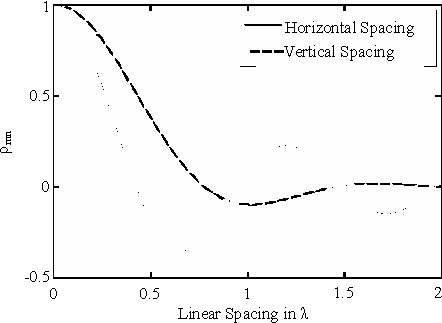
\includegraphics[scale=1.2]{img/analysis/mimoSpacing}
  \caption{Spacing versus wavelength for the horizontal and vertical case\cite{Tim2012Practical}}
  \label{fig:mimo-spacing}
\end{figure}

\subsubsection{Polarization and Radiation Patterns}
In addition to the spatial separation to decorrelate antennas, polarization and different radiation patterns can also be used to decorrelate elements. This is very often used in small mobile devices where the physical size limits the spacing between elements.  

In theory, using a perfectly polarized dipole and loop antenna, it would be possible to create totally decorrelated elements because they have opposite polarization. This is hard to implement in practice, but it is possible to lower the correlation of to elements by having a difference in polarization. However, using different polarization to get a lower correlation requires a suitable XPR in the channel. The XPR should be around \SI{6}{dB} or lower\cite{Tim2012Practical}. 

\subsubsection{Multiplexing Efficiency}
\label{sec:muxefficiency}

Multiplexing efficiency is a measure of total efficiency for an antenna system, taking into account the total efficiency for each antenna \emph{and} the correlation between antenna elements. In this way, it is a single parameter that describes the total loss in SNR (or power) when using a MIMO antenna system \cite{tian2011multiplexing}.

For a $2\times2$ MIMO system, relevant to this project, and assuming high SNR, the multiplexing efficiency, $\eta_{\text{mux}}$, is computed as \cite{tian2011multiplexing}
\begin{equation} %%%%
    \eta_{\text{mux}} = \sqrt{\eta_1 \eta_2 (1 - |\rho|^2)}
\end{equation}
where
\begin{where}
\item[$\eta_n$] Total efficiency of the $n$th antenna.
\item[$\rho$] Correlation between antenna 1 and 2.
\end{where}

In the rest of the report, efficiency and correlation will mostly be treated separately to see more details between the antennas. However, the metric of multiplexing may be useful when evaluating the antennas performance in a link budget.
